\documentclass[oneside]{amsart}

\usepackage{microtype}
\usepackage[english]{babel}

\usepackage{amsmath}
\usepackage{amsthm}

\newtheorem{theorem}{Theorem}
\newtheorem{corollary}[theorem]{Corollary}
\newtheorem{proposition}[theorem]{Proposition}
\newtheorem{lemma}[theorem]{Lemma}
\newtheorem{conjecture}[theorem]{Conjecture}
\theoremstyle{definition}
\newtheorem{definition}[theorem]{Definition}
\newtheorem{example}[theorem]{Example}
\newtheorem{remark}[theorem]{Remark}

\usepackage{amssymb}
\usepackage{mathtools}
\usepackage[unicode=true,hidelinks,bookmarksnumbered]{hyperref}
\usepackage{enumitem}

\setlist{noitemsep}
\setlist[enumerate]{label=(\arabic*), font=\upshape}

\usepackage{tikz}

\usetikzlibrary{babel}
\usetikzlibrary{matrix}
\usetikzlibrary{arrows}
\usetikzlibrary{calc}
\usetikzlibrary{cd}
\usetikzlibrary{positioning}
\usetikzlibrary{decorations.markings}
\usetikzlibrary{svg.path}
\tikzset{ampersand replacement=\&}

\usepackage[style=alphabetic,maxbibnames=99,maxalphanames=5]{biblatex}

\renewcommand*{\labelalphaothers}{\textsuperscript{+}}
\DeclareFieldFormat*{title}{\mkbibemph{#1}}
\addbibresource{stp.bib}

\usepackage{csquotes}

% Skeleton of a simplicial complex
\DeclareMathOperator\skel{skel}
% Colimit of a functor
\DeclareMathOperator\colim{colim}
% Kernel of an object
\DeclareMathOperator\Ker{Ker}
% Object class of a category
\DeclareMathOperator\Ob{Ob}
% Hom-set of a category
\DeclareMathOperator\Hom{Hom}
% Leading simplex
\DeclareMathOperator\LS{LS}
% Used in subscripts of categories
\newcommand\lex{\mathrm{lex}}
\newcommand\grlex{\mathrm{grlex}}
\newcommand\ord{\mathrm{ord}}
% Category of simplicial complexes
\newcommand\Simp{\operatorname{Simp}}
% Category of sets
\newcommand\Set{\operatorname{Set}}
% Category of #1-modules
\newcommand\Mod[1]{\operatorname{Mod}_{#1}}
% Principal persistent set
\newcommand\pt{\mathrm{pt}}
% Support of persistence module
\DeclareMathOperator\Supp{Supp}

\begin{document}
\title[Cofiltrations of spanning trees]{Cofiltrations of spanning trees in multiparameter persistent homology}
\subjclass[2020]{Primary 55N31; secondary 05C50, 05C90}
\author{Fritz Grimpen}
\email{grimpen@uni-bremen.de}
\address{Institute for Algebra, Geometry, Topology and its Applications (ALTA), Department of Mathematics, University of Bremen, Germany}
\author{Anastasios Stefanou}
\email{stefanou@uni-bremen.de}
\address{Institute for Algebra, Geometry, Topology and its Applications (ALTA), Department of Mathematics and Computer Science, University of Bremen, Germany}
\keywords{Cofiltrations, Spanning Trees, Multiparameter Persistent Homology}
\begin{abstract}
    Given a multiparameter filtration of simplicial complexes, we consider the problem of explicitly constructing generators for the multipersistent homology groups with arbitrary PID coefficients.
    We propose the use of spanning trees as a tool to identify such generators by introducing a condition for persistent spanning trees, which is accompanied by an existence result for cofiltrations consisting of spanning trees.
    We also introduce a generalization of spanning trees, called spanning complexes, for dimensions higher than one, and we establish their existence as a first step towards this direction.
\end{abstract}
\maketitle

\tableofcontents

\section{Introduction}
Persistent homology studies the evolution of topological features of a dataset (finite metric space) across a given filtration on the dataset \cite{EdelsbrunnerLetscherZomorodian2002}. 
It is arguably the most heavily used tool in Topological Data Analysis (TDA) \cite{Carlsson2009,EdelsbrunnerHarer2010}.~Persistent homology has the algebraic structure of an $\mathbb{N}$-graded module \cite{CarlssonZomorodianCollinsGuibas2005}.
 
\subsection{Multiparameter persistence} Persistent homology extends naturally from one-parameter filtrations \cite{ZomorodianCarlsson2005} to multiparameter filtrations of datasets \cite{CarlssonZomorodian2009}. The corresponding algebraic structure of multiparameter homology is that of an $\mathbb{N}^d$-graded module, as shown in \cite{CarlssonZomorodian2009}.
In fact persistent homology can be defined for filtrations parameterized over any poset $Q$ \cite{BubenikScott2014}.
The extension from graded modules to multigraded modules is of particular importance to TDA, since there are situations where important information from data cannot be captured from persistent homology by merely considering one-parameter filtration, e.g.~persistent homology is shown to be unstable to the presence of outliers \cite{CarlssonZomorodian2009,LesnickWright2015}.~By introducing a density parameter as a second filtration parameter on datasets, outliers in datasets can then be regarded as noise, making two-parameter persistent homology robust to the presence of outliers in the data. Thus, additional information from datasets can be extracted from datasets by studying multiparameter persistent homology.   
In multiparameter persistence, in general, there is no way to visualize the indecomposable modules as interval modules \cite{CarlssonZomorodian2009, DeyXin2022}, as in the case of one-parameter persistence \cite{BotnanCrawley-Boevey2020,Crawley-Boevey2015}. 
Therefore, recent research works in multipersistence theory have been focusing on the study of multipersistent invariants \cite{KimMemoli2021,Patel2018}.

\subsection{Minimal presentations}The key techniques to better understand the structure of multiparameter persistence modules as well as to help towards an efficient computation of multipersistent invariants of modules, are the minimal free presentations, minimal free resolutions  \cite{CoxLittleOShea2005}, and the recently introduced  minimal flat-injective presentations \cite{Miller2020a} of multigraded modules. 
However, in practice, all of these techniques often pre-assume that the module is equipped with a set of generators to begin with, and that the  multigraded module is a submodule of some given free module.
Gröbner basis methods can then be utilized to compute a minimal presentation and a minimal free resolution of the module \cite{CoxLittleOShea2005,LaScalaStillman1998,MillerSturmfels2005}.
As of now, the problem of finding an efficient way to compute a minimal presentation of multiparameter persistence modules remains open. 
Some works in TDA towards this direction include \cite{CarlssonSinghZomorodian2010,ChachólskiScolamieroVaccarino2017,LesnickWright2022}.

\subsection{Related work}
In \cite{CarlssonSinghZomorodian2010} the authors show that if a multifiltration $X = (X_a)_{a \in \mathbb N^d}$ is one-critical, i.e.~every simplex enters the multifiltration in at most one multidegree (thereby making each $C_n(X)$ a free module), then Schreyer's algorithm \cite{CoxLittleOShea2005} can be directly applied for computing a Gröbner basis for the $n$-cycle module $Z_n(X)=\Ker \partial_n$ of the homology module $H_n(X)=\Ker \partial_n / \operatorname{Im}\partial_{n+1}$ of a multifiltration $X$, and thus for computing a minimal free presentation for the homology module.
In \cite{ChachólskiScolamieroVaccarino2017}, the authors attempted to describe in an explicit and combinatorial way the multigraded module structure of the homology of any multifiltration of simplicial complexes.
They developed a construction that realizes the $n$-th homology module $H_n(X)$ of a multifiltration $X$, as the homology  $\Ker f/\operatorname{Im} g$ of a certain chain complex  $F_1\xrightarrow{f}F_2\xrightarrow{g}F_3$ of free multigraded modules.
They also proved that the multigraded modules that can occur as $R$-spans of multifiltrations of sets are the direct sums of monomial ideals. 

In the case of a $2$-parameter filtration $X$, they  construct a free presentation 
\[ F_1\to F_0\to H_n(X)\to 0 \]
for the homology module $H_n(X)$, where $F_1$ is explicitly defined and $F_0$ is the kernel of a  morphism between certain free modules.
However, that kernel module $F_0$, although free, was not defined explicitly, as mentioned by the authors, and therefore there was not an explicit method given for computing a (minimal) free presentation for $H_n(X)$.
The issue was later resolved in \cite{LesnickWright2022}, where the authors devised a general algorithm for computing minimal presentation for $2$-parameter persistence modules (also called bigraded modules), whenever they are represented as $M\cong \Ker g/\operatorname{Im} g$ (for instance via the combinatorial presentation of \cite{ChachólskiScolamieroVaccarino2017}), for some chain complex of free $2$-parameter persistence modules $F_1\xrightarrow{f}F_2\xrightarrow{g}F_3$.
In both works, for $d=2$, the authors are invoking the algebraic-geometric fact that over two variables ($2$-parameters), kernels of free bigraded modules are also free.
This is no longer true when we work on multigraded modules over $d\geq3$ parameters.

\subsection{Motivation}
Our goal is to develop a method for computing (minimal) generators for the homology of a multifiltration.
Our work is motivated by the problem of computing generators of kernels of morphisms of \emph{upper-set decomposable} modules (direct sums of monomial ideals) as in \cite{ChachólskiScolamieroVaccarino2017}.
However, in this work our approach is to investigate a way to find (minimal) free generators for the $n$-cycle module $Z_n(X)$ of a multifiltration $X$, since this would be enough for our goal.
Indeed, if we know the generators of $Z_n(X)$, because of the canonical epimorphism from $Z_n(X)$ onto $H_n(X)$, we will also obtain free generators for $H_n(X)$.
This will then enable us, at least implicitly, to be able to apply the machinery of commutative algebra to compute a minimal free presentation and a minimal free resolution of the homology of a multifiltration. 
In the static case of simplicial complexes, we can compute the generators of the first homology group $H_1(X)$ of a given complex $X$ by using spanning tree subcomplexes $T$ of $X$.
We have the following theorem which is known from many sources in the literature.
 
\begin{theorem}[\cite{Kozlov2020,Spanier1982}]
    If $X$ is a 1-dimensional simplicial complex and $T$ a spanning tree of $X$, then $H_1(X) \cong C_1(X, T)$.
\end{theorem}

\subsection{Our contributions}

The main contribution of this work is a method to construct generators of the $1$-dimensional cycle module $Z_1(X; R) = \Ker \partial_1$ for a given multifiltration $X = (X^q)_{q \in Q}$ of finite simplicial complexes over a finite poset $Q$ and an arbitrary principal ideal domain $R$.
To the multifiltration $X$ we associate a \emph{cofiltration of spanning trees} $T = (T^q)_{q \in Q}$ by endowing the simplicial complex $\bigcup_{q \in Q} X^q$ with a simplicial order.
We show that these multifiltrations satisfy the following crucial property.
\begin{theorem}
    \label{theorem:IntroMainResult}
    For any poset $Q$ and any $Q$-indexed filtration $X = (X^q)_q$ of simplicial complexes, there exists a $Q$-indexed filtration $T = (T^q)_q$ of spanning trees of $X$ satisfying $X^q \setminus T^q \subseteq X^{q'} \setminus T^{q'}$ for any pair $q \leq q'$ in $Q$.
\end{theorem}

This existence result for a cofiltration of spanning trees $T$ associated to $X$ allows us to associate to every edge $\sigma$ contained in $X$ but not in $T$ an upper-set decomposable module $M_\sigma$.
We show that the direct sum $\bigoplus_\sigma M_\sigma$, where $\sigma$ ranges over any edge $\sigma$ in $X$ but not in $T$, admits a canonical epimorphism of persistence modules onto $Z_1(X)$, and subsequently onto $H_1(X)$.
\begin{theorem}
    Let $Q$ be any finite poset and $X = (X^q)_{q \in Q}$ a $Q$-indexed filtration of finite simplicial complexes.
    Then, given a choice of simplicial order on $X$ there exists an epimorphism $\varphi_1\colon M \to Z_1(X)$, where $M$ is an upper set decomposable module, constructed explicitly from the cofiltration of order-minimal spanning trees.
\end{theorem}

As a last step and in order to generalize that technique to higher homology groups $H_n(X)$, $n \in \mathbb N$, we introduce a direct generalization of spanning trees to higher dimensions.
We call this generalized structure an \emph{$n$-spanning complex} and show the existence by an application of Zorn's lemma.

\begin{theorem}
    For any simplicial complex~$X$ and any $n \in \mathbb N$ there exists a subcomplex $A$ such that $Z_n(A) = 0$ and $B_{n-1}(A) = B_{n-1}(X)$, i.e.\ $X$ admits an $n$-spanning complex.
\end{theorem}

\subsection{Organization}
In Section~\ref{section:Preliminaries}, we recall the basic definitions of partially ordered sets, simplicial complexes, simplicial homology, persistence modules, and persistent simplicial homology.
In Section~\ref{section:SpanningTrees}, we define our notion of spanning trees in terms of the boundaries and chains of subcomplexes.
Subsequently, we state an edge-exchange lemma (Lemma~\ref{lemma:STEdgeExchange}) and the existence of a classical isomorphism associated to spanning trees (Theorem~\ref{theorem:SpanningTreeMain}).

In Section~\ref{section:CofiltrationsOfSpanningTrees}, we investigate the previously introduced notion of spanning trees on their behavior under persistence.
In order to describe this behavior, we introduce the notion of a cofiltration of spanning trees (Definition~\ref{definition:CofST}) and prove that they always exist for finite posets and (globally) finite filtrations (Theorem~\ref{theorem:MainResult}).

The Section~\ref{section:RSpans} is used to collect a variety of algebraic statements concerning so-called $R$-spans of set-valued diagrams over any small category.
These results are meant to be used in Section~\ref{section:GeneratingH1}, where we construct from a cofiltration of spanning trees an upper set decomposable persistence module that enjoys an epimorphism onto the first persistent homology group (Theorem~\ref{theorem:GenH1}).

The last section, Section~\ref{section:HigherDimensionalSpanningSubcomplexes}, is meant as an outlook to analogue results for higher-dimensions.
We introduce the generalized notion of $n$-spanning complexes and show that their existence follows from Zorn's lemma (Theorem~\ref{theorem:ExistenceNSS}).

\section{Preliminaries}%
\label{section:Preliminaries}

Throughout this paper, let $R$ be a principal ideal domain.

Let $Q$ be a non-empty set.
Recall that a \emph{partial order} on $Q$ is a relation $\mathord\leq \subseteq Q \times Q$, where $(q, q') \in \mathord\leq$ is denoted by $q \leq q'$, satisfying the following three properties for all $q, q', q'' \in Q$:
\begin{enumerate}[label=(\roman*)]
    \item $q \leq q$ (\emph{Reflexivity}).
    \item $q \leq q'$ and $q' \leq q''$ imply $q \leq q''$ (\emph{Transitivity}).
    \item $q \leq q'$ and $q' \leq q$ imply $q = q'$ (\emph{Antisymmetry}).
\end{enumerate}
If $\mathord\leq$ satisfies also $q \leq q'$ or $q' \leq q$ for $q, q' \in Q$, then $\mathord\leq$ is called a \emph{total order}.
We call the pair $(Q, \mathord\leq)$ a \emph{poset} whenever $\mathord\leq$ is a partial order.
Moreover, if $\mathord\leq$ is a total order, then we call $(Q, \mathord\leq)$ a \emph{totally ordered set}.
A set $X$ is said to be \emph{well-ordered} by a partial order $\leq$ if every non-empty subset of $X$ admits a unique minimal element.
Then, $\leq$ is called a \emph{well-ordering} of $X$, and we denote by $\min(A)$ the unique minimal element of $A$ for $A \subseteq X$.
In particular, every well-ordering of $X$ is a total order on $X$.

\subsection{Simplicial homology}

Let $V$ be a non-empty set, which we call the \emph{vertex set} and whose elements are called \emph{vertices}.
An \emph{(abstract) simplicial complex} (over $V$) is a subset $X$ of the power set of $V$ such that
\begin{enumerate}[label=(\roman*)]
    \item every element $\sigma \in X$ is a finite subset of $V$ and
    \item for every element $\sigma \in X$ every subset $\tau$ of $\sigma$ is also an element of $X$, i.e.\ $\sigma \in X$ and $\tau \subseteq \sigma$ imply $\tau \in X$.
\end{enumerate}
The elements of $X$ are called \emph{simplices}.
For $n \in \mathbb N$ we denote by $X_n$ the simplices in $X$ of cardinality equal to $n + 1$, and we define the \emph{$n$-skeleton of $X$} by $\skel_n X = \bigcup_{k \leq n} X_k$.
Although the vertex set $V$ is part of the simplicial complex $X$, we omit it unless it is necessary, and then we denote it by $V(X)$.
Given simplicial complexes $X$ over $V$ and $Y$ over $W$, a map $f\colon V \to W$ is a \emph{simplicial map} if for $\sigma = \{ v_0, \dotsc, v_n \} \in X$ it holds $f(\sigma) = \{ f(v_0), \dotsc, f(v_n) \} \in Y$.
We also write $f \colon X \to Y$ for a simplicial map.
Simplicial complexes with simplicial maps constitute the category $\Simp$ of simplicial complexes.

For the purposes of (simplicial) homology, the vertex set $V(X)$ of a simplicial complex $X$ is endowed with a fixed total order $\preceq$.
We shall extend this idea to the whole simplicial complex by endowing a simplicial complex $X$, viewed as its set of simplices, with a fixed well-ordering $\preceq$:
The pair $(X, \mathord\preceq)$ is an \emph{ordered simplicial complex} and $\preceq$ is a \emph{simplicial order} in this context.
Note that an ordered simplicial complex $(X, \mathord\preceq)$ induces a total order on the vertex set $V(X)$ by the correspondence $V \leftrightarrow \{ \{ v \} \mid v \in V \}$.
We write $[v_0, \dotsc, v_n]$ to denote the simplex $\{ v_0, \dotsc, v_n\}$ if $v_0 \leq \dotsb \leq v_n$.

Let $(X, \mathord\preceq_X)$ and $(Y, \mathord\preceq_Y)$ be ordered simplicial complexes and let $f\colon X \to Y$ a simplicial map.
Then, we say that $f$ is a \emph{morphism of ordered simplicial complexes} or a \emph{order-preserving simplicial map} if, for all $\sigma, \tau \in X$ satisfying $\sigma \preceq_X \tau$, it follows $f(\sigma) \preceq_Y f(\tau)$.
We denote the category with ordered simplicial complexes as objects and order-preserving simplicial maps by $\Simp_\ord$ and call it the \emph{category of ordered simplicial complexes}.

The category of simplicial complexes admits a (topological) homology theory, namely \emph{simplicial homology}, see~\cite{Hatcher2015, Spanier1982}.
Let $X$ be a simplicial complex and let $V(X)$ be endowed with a total order~$\leq$.
For a simplex $[v_0, \dotsc, v_n]$ we write $[v_0, \dotsc, \widehat{v_i}, \dotsc, v_n]$ to denote the simplex $\{ v_0, \dotsc, v_n \} \setminus \{ v_i \}$.

For $n \in \mathbb N$, let $C_n(X)$ be the free $R$-module generated by the $n$-simplices $X_n$ and let
\begin{align*}
    \partial_n\colon C_n(X) &\longrightarrow C_{n-1}(X) \text, \\
    [v_0, \dotsc, v_n] &\longmapsto \sum_{i = 0}^n (-1)^n [v_0, \dotsc, \widehat{v_i}, \dotsc, v_n] \text,
\end{align*}
be the \emph{boundary homomorphism} defined on generators of $C_n(X)$.
The boundary homomorphisms satisfy $\partial_n \circ \partial_{n+1} = 0$, and the quotient $\Ker \partial_n/\operatorname{Im} \partial_{n+1}$ is the \emph{$n$-th (simplicial) homology module}, which is denoted by $H_n(X)$.
Additionally, we define $Z_n(X) = \Ker \partial_n$ and $B_n(X) = \operatorname{Im} \partial_{n+1}$.
We note that $Z_n(X)$ and $B_n(X)$ are free since $R$ is a PID by assumption.

\subsection{Persistence modules and persistent homology}

Let $(Q, \mathord\leq)$ be a poset.
A family $(X^q)_{q \in Q}$ of simplicial complexes is called a \emph{filtration} if for all $q, q' \in Q$ with $q \leq q'$ it holds $X^q \subseteq X^{q'}$.
Note that $X^{q'} \subseteq \bigcup_{q \in Q} X^q$ for every $q' \in Q$.
For each $n \in \mathbb N$, every pair $q, q' \in Q$ with $q \leq q'$ induces a homomorphism of $R$-modules
\[ H_n(X^q \subseteq X^{q'})\colon H_n(X^q) \longrightarrow H_n(X^{q'}) \text. \]
The collection $(H_n(X^q))_{q \in Q}$ together with these homomorphisms $H_n(X^q \subseteq X^{q'})$ for all pairs $q, q' \in Q$ satisfying $q \leq q'$ is called the \emph{$n$-th persistent homology module of $(X^q)_{q \in Q}$}.
The underlying algebraic structure is a \emph{persistence module}.

Given a poset $(Q, \mathord\leq)$, we can consider its associated \emph{poset category} $\mathcal Q$ that is given by
\[ \Ob(\mathcal Q) = Q \text, \qquad \Hom_{\mathcal Q}(q, q') = \{ (q, q') \} \cap \mathord\leq \text. \]
We denote the associated poset category of $Q$ also by $Q$.

Further, denote by $\Mod{R}$ the category of $R$-modules.
Then, a \emph{persistence module} with coefficients in $R$ and indexed over $Q = (Q, \mathord\leq)$ is a functor $M\colon Q \to \Mod{R}$.
The images of morphisms in $Q$ under a persistence module are called the \emph{structure homomorphisms} of $M$.
The morphisms of persistence modules $M, N\colon Q \to \Mod{R}$ are precisely the natural transformations $M \to N$ .
More generally, a persistence module can be indexed by an arbitrary small category $I$, e.g.\ $I = \mathcal Q$ the posetal category associated to $(Q, \mathord\leq)$.
We write $\Mod{R}^I$ to denote the \emph{category of persistence modules} indexed by the small category $I$.
By abusing notation, we shall write $\Mod{R}^Q$ to denote the category of persistence modules indexed by the posetal category associated to $(Q, \mathord\leq)$.

Furthermore, we call a set-valued functor on $Q$ a \emph{persistent set} and a corresponding natural transformation a \emph{persistent map}.
The category of persistent sets is denoted by $\Set^Q$.

\section{Spanning trees of simplicial complexes}%
\label{section:SpanningTrees}

Traditionally, spanning trees of graphs are subgraphs that reflect the connectivity properties of the original graph while preserving acyclicity and means to identify cyclic paths in a graph \cite{BondyMurty2008,Kozlov2020,Lovász1977}.
As such, they are classically characterized in terms of combinatorial properties on them.
We modify the standard definition of a spanning tree to facilitate the need of having an algebraic characterization in the following way:
\begin{itemize}
    \item We characterize spanning trees in terms of their cycle and boundary modules of simplicial homology, see Definition~\ref{definition:SpanningTree} below.
    \item The zeroth homology module of a spanning tree does not need to trivialize, i.e.\ a spanning tree is not necessarily connected.
\end{itemize}

Throughout this section, let $X$ be a simplicial complex with vertex set $V$.

\begin{definition}[Spanning tree]%
    \label{definition:SpanningTree}
    A \emph{spanning tree} of~$X$ is a simplicial subcomplex $T$ of $X$ such that
    \begin{enumerate}[label=(\roman*)]
        \item\label{definition:SpanningTree:c1} $X_0 = T_0$,
        \item\label{definition:SpanningTree:c2} the boundary homomorphism $\partial_1\colon C_1(T) \to C_0(T)$ is injective, and
        \item\label{definition:SpanningTree:c3} $B_0(X) = B_0(T)$.
    \end{enumerate}
\end{definition}

The first condition states the natural assumption that any spanning tree of $X$ needs to have the same vertices (in the sense of 0-simplices) as $X$.
Further, the second condition requires that any spanning tree of $X$ is indeed a tree, i.e.\ the 1-dimensional cycle module of any spanning tree is trivial.

The most useful condition is the third, which roughly states that a spanning tree indeed spans the space $X$ in the following sense:
Suppose that $T$ is a spanning tree of $X$ and let $u, v$ be vertices of $X$.
Further, suppose that there exists a path in $X$ from $u$ to $v$, i.e.\ $u$ and $v$ lie in the same path component of $X$, or equivalent there is a 1-chain $c \in C_1(X)$ such that $\partial_1 c = u - v$.
Then, the third condition implies that there exists a 1-chain $c' \in C_1(T)$ such that $\partial_1 c = \partial_1 c' \in B_0(T)$.
Thus, both vertices $u$ and $v$ also lie in the same path component of $T$.

More generally, if $c$ is a 1-chain in $X$, then there always exists a 1-chain~$c'$ in $T$ such that $c - c'$ is a cycle.
Particularly, it follows from Definition~\ref{definition:SpanningTree} \ref{definition:SpanningTree:c2} that the chain $c' \in C_1(T)$ is uniquely determined by $c \in C_1(X)$.

We are now developing the basic theory of (homological) spanning trees as above.
To that end, we fix the following notation:
For sets $X$, $Y$, and $Z$ we write $X \cup Y \setminus Z$ to denote $(X \cup Y) \setminus Z$.
That is, the set difference and union operators have the same precedence and are left-associative.

Let $T$ be a spanning tree of $X$.
We pick some edge (1-simplex)~$e$ in $X$ that is not in $T$ and we ask whether there exists another spanning tree of $X$ that actually contains $e$.
It is clear that $A = T \cup \{ e \}$ still satisfies $B_0(X) = B_0(A)$ and $V(X) = V(A)$, and thus the subcomplex $A$ still satisfies two out of three conditions for a spanning tree, see Definition~\ref{definition:SpanningTree} \ref{definition:SpanningTree:c1} and \ref{definition:SpanningTree:c3}.
However, it is also easy to see that $Z_1(A) \neq 0$.
Thus, $A$ does not satisfy the acyclicity condition of spanning trees.

Therefore, the actual question is whether we can find some edge $e'$ in $T$ such that $T \cup \{ e \} \setminus \{ e' \}$ is again a spanning tree.
We call the following the lemma the \emph{edge-exchange lemma}.
A similar statement about spanning trees is known as the \emph{tree exchange property}, see \cite[p.\ 113, Exercise 4.3.2]{BondyMurty2008}.

\begin{lemma}%
    \label{lemma:STEdgeExchange}
    Let $T$ be a spanning tree of the simplicial complex~$X$.
    Then, for every edge~$\sigma \in X$ that is not contained in $T$, there exists an edge $\tau \in T$ such that $T \cup \{ \sigma \} \setminus \{ \tau \}$ is a spanning tree of~$X$.

    Moreover, if $c$ is a 1-chain in $T$ such that $\partial_1 c = \partial_1 \sigma$, then every simplex in $c$ is admissible as $\tau$.

    \begin{proof}
        Let $\sigma$ be an edge contained in $X$ but not in $T$.
        Since $T$ is a spanning tree, we find a 1-chain $c$ in $T$ such that $\partial_1 c = \partial_1 \sigma$.
        Moreover, we can choose $\lambda_0, \dotsc, \lambda_k \in \{ 1, -1 \}$ and distinct edges $\tau_0, \dotsc, \tau_k \in T$ such that $c = \sum_{i = 0}^k \lambda_i \tau_i$.
        We set $\tau = \tau_0$, i.e.\ $c = \lambda_0 \tau + \sum_{i = 1}^k \lambda_i \tau_i$.
    
        Let $b \in B_0(X)$.
        Then, we can choosse a 1-chain $c' = \mu_0 \tau + \sum_{i = 1}^l \mu_i \sigma_i$ in $T$ such that $\partial_1 c' = b$, where the simplices $\tau, \sigma_1, \dotsc, \sigma_k$ are distinct.
        By replacing $\tau$ in $c'$ with the 1-chain $\sum_{i = 1}^k \lambda_i \tau_i - \sigma$, which is contained in $X \setminus T$, we obtain the chain
        \[ c'' = \sum_{i = 1}^k \mu_0 \lambda_i \tau_i - \mu_0 \sigma + \sum_{i = 1}^k \mu_i \sigma_i \text. \]
        Since the chains $\sum_{i = 1}^k \lambda_i \tau_i$ and $\sigma$ have the same boundary, the boundary of $c''$ coincides with the boundary of $c'$.
        Further, the chain $c''$ is, by construction, contained in $T'$.
        Hence, $\partial_1 c'' = \partial_1 c' = b \in B_0(T')$.
        Since $T' \subseteq X$, this proves in particular $B_0(X) = B_0(T')$ and $B_0(T) = B_0(T')$.
    
        Let $z \in Z_1(T + \sigma - \tau)$ and choose $\mu_0, \mu_1, \dotsc, \mu_l \in R$ and edges $\tau_1, \dotsc, \tau_l$ distinct from $\tau$ in $T$ such that $z = \mu_0 \sigma + \sum_{j = 1}^l \mu_j \tau_j$.
        Then, we have $\mu_0 \neq 0$ unless $z = 0$.
        Therefore, we assume that $z \neq 0$.
        
        Then, we have
        \[ \mu_0 (u - v) = \mu_0 \partial_1 \sigma = -\partial_1 \sum_{j = 1}^l \mu_j \tau_j  \]
        for vertices distinct $u$ and $v$ in $X$.
        Furthermore, $\mu_0 \neq 0$ is invertible since there exists some chain $c \in C_1(T)$ satisfying $\partial_1 c = u - v$ and $\sum_{j = 1}^l \mu_j \tau_j = \mu_0 c$ by the injectivity of $\partial_1$ on $C_1(T)$.
        Thus, $u - v = -\partial_1 \sum_{j = 1}^l \mu_j \mu_0^{-1} \tau_j$.
        
        However, this means that some of the $\tau_1, \dotsc, \tau_j$ must coincide with $\tau$ by construction.
        This is a contradiction to the assumption that $\tau_1, \dotsc, \tau_j$ are distinct from $\tau$.
        Hence, $Z_1(T + \sigma - \tau) = 0$.
    \end{proof}    
\end{lemma}

We call a pair $(\sigma, \tau)$ of an edge $\sigma \in X \setminus T$ and an edge $\tau \in T$ an \emph{edge exchange pair} if $T \cup \{ \sigma \} \setminus \{ \tau \}$ is a spanning tree.
For notational convenience, we write $T + \sigma - \tau$ for the set $T \cup \{ \sigma \} \setminus \{ \tau \}$.

We have seen that every edge that is not contained in a spanning tree induces a cycle, where exactly one edge in this cycle is not contained in the spanning tree.
The following theorem, which is known for a long time, states that the cycles induced by edges not contained in a spanning tree are precisely the generators of the $1$-dimensional cycle group of the spanned simplicial complex.
Proofs of this and equivalent results can be found in \cite[Theorem~1.9.4]{Diestel2017}, \cite[Theorem~2.33]{Kozlov2020}, and \cite[Theorem~3, p.\ 140]{Spanier1982}.

\begin{theorem}%
    \label{theorem:SpanningTreeMain}
    Let $T$ be a spanning tree of $X$.
    Then, the homomorphism
    \[ j\colon Z_1(X) \longrightarrow C_1(X, T) \text, \quad z \longmapsto z + C_1(T) \text, \]
    is an isomorphism of $R$-modules.

    \begin{proof}
        Let $z \in Z_1(X)$ such that $z \in C_1(T)$.
        Then, $z = 0$ by $Z_1(T) = 0$.
        Hence, $j$ is a monomorphism.
    
        In order to prove the surjectivity of $j$, let $c \in C_1(T)$.
        By $B_0(T) = B_0(X)$, we find $c' \in C_1(T)$ such that $\partial_1 c = \partial_1 c'$, that is~$c - c' \in Z_1(X)$.
        Then, we have
        \[ j(c - c') = c - c' + C_1(T) = c + C_1(T) \]
        since $c' \in C_1(T)$.
        Thus, the homomorphism~$j$ is surjective, and it follows $Z_1(X) \cong C_1(X, T)$.
    \end{proof}
\end{theorem}

Next, we are considering the notion of spanning trees of ordered simplicial complexes.
We assume that any ordered simplicial complex $(X, \mathord\preceq)$ satisfies the following properties:
\begin{enumerate}[label=(\roman*)]
    \item The total order~$\mathord\preceq$ is a well-order, i.e.\ every subset $A$ of $X$ admits a minimal element.
    \item If $\sigma$ is a simplex of $X$ and $\tau$ a face of $\sigma$, then $\tau \preceq \sigma$.
\end{enumerate}

It turns out that every finite, ordered simplicial complex admits a special, distinguished spanning tree that is minimal in a certain sense w.r.t.\ the well-ordering~$\preceq$.
We characterize these spanning trees using lexicographic orders.

\begin{definition}[Lexicographic orders]
    Let $(X, \mathord\preceq)$ be a well-ordered set, e.g.\ $(X, \mathord\preceq)$ is an ordered simplicial complex.
    The \emph{lexicographic order}~$\mathord\preceq_\lex$ on $2^X$ is given by
    \[ A \preceq_\lex B \iff A = B \text{ or } \min((A \setminus B) \cup (B \setminus A)) \in A \]
    for subsets $A, B \subseteq X$.
\end{definition}

\begin{remark}
    Let $A, B \subseteq X$, where $X$ is an arbitrary well-ordered set~$X$.
    Then, $A \preceq_\lex B$ if and only if there exists $x \in A \setminus B$ such that for every $y \in (A \setminus B) \cup (B \setminus A)$ it holds $x \preceq y$.
\end{remark}

\begin{lemma}%
    \label{lemma:LexTotalOrder}
    The lexicographic order~$\preceq_\lex$ is a total order.
\end{lemma}

\begin{remark}
    If $X$ is a finite set, its power set~$2^X$ is also finite, and then the lexicographic order~$\preceq_\lex$ is a well-ordering of $2^X$.
\end{remark}

\begin{example}
    Consider the totally ordered set $X = \{ 1 < 2 < 3 \}$ and endow its powerset
    \[ 2^X = \{ \emptyset, 1, 2, 3, 12, 13, 23, 123 \} \]
    with the lexicographic order $<_\lex$, where we denote the subsets of $X$ as words, e.g.\ $12 = \{ 1, 2 \}$.
    Then it holds $12 <_\lex 13 <_\lex 23$.
    This motivates the term \enquote{lexicographic order} for the order defined above.

    See Figure~\ref{figure:123LexOrder} for a table of all relations in $2^X$.
    We note that $A \subseteq B$ implies $B <_\lex A$ and therefore the element $\emptyset$ is maximal. Analogously, $X \in 2^X$ is minimal w.r.t.\ the lexicographic order.

    When we compare this to the graded lexicographic order $<_\grlex$, see Figure~\ref{figure:123GrLexOrder}, we note that $\emptyset$ is minimal and $X$ is maximal w.r.t.\ the graded lexicographic order.
\end{example}

\begin{figure}
    \centering
    \begin{tabular}{r|cccccccc}
                    & $\emptyset$ & $1$    & $2$    & $3$    & $12$   & $13$   & $23$   & $123$  \\ \hline
        $\emptyset$ & $=$         & $\geq$ & $\geq$ & $\geq$ & $\geq$ & $\geq$ & $\geq$ & $\geq$ \\
        $1$         &             & $=$    & $\leq$ & $\leq$ & $\geq$ & $\geq$ & $\leq$ & $\geq$ \\
        $2$         &             &        & $=$    & $\leq$ & $\geq$ & $\geq$ & $\geq$ & $\geq$ \\
        $3$         &             &        &        & $=$    & $\geq$ & $\geq$ & $\geq$ & $\geq$ \\
        $12$        &             &        &        &        & $=$    & $\leq$ & $\leq$ & $\geq$ \\
        $13$        &             &        &        &        &        & $=$    & $\leq$ & $\geq$ \\
        $23$        &             &        &        &        &        &        & $=$    & $\geq$ \\
        $123$       &             &        &        &        &        &        &        & $=$
    \end{tabular}

    \caption{The relations of the lexicographic order on $2^X$ for $X = \{ 1 < 2 < 3 \}$, where the entry \enquote{$\geq$} denotes \enquote{$\text{row label} \geq \text{column label}$} and the entry \enquote{$\leq$} denotes \enquote{$\text{row label} \leq \text{column label}$}.}
    \label{figure:123LexOrder}
\end{figure}

\begin{figure}
    \centering
    \begin{tabular}{r|cccccccc}
                    & $\emptyset$ & $1$    & $2$    & $3$    & $12$   & $13$   & $23$   & $123$  \\ \hline
        $\emptyset$ & $=$         & $\leq$ & $\leq$ & $\leq$ & $\leq$ & $\leq$ & $\leq$ & $\leq$ \\
        $1$         &             & $=$    & $\leq$ & $\leq$ & $\leq$ & $\leq$ & $\leq$ & $\leq$ \\
        $2$         &             &        & $=$    & $\leq$ & $\leq$ & $\leq$ & $\leq$ & $\leq$ \\
        $3$         &             &        &        & $=$    & $\leq$ & $\leq$ & $\leq$ & $\leq$ \\
        $12$        &             &        &        &        & $=$    & $\leq$ & $\leq$ & $\leq$ \\
        $13$        &             &        &        &        &        & $=$    & $\leq$ & $\leq$ \\
        $23$        &             &        &        &        &        &        & $=$    & $\leq$ \\
        $123$       &             &        &        &        &        &        &        & $=$
    \end{tabular}

    \caption{The relations of the graded lexicographic order on $2^X$ for $X = \{ 1 < 2 < 3 \}$, where the entry \enquote{$\leq$} means \enquote{$\text{row label} \leq \text{column label}$}.}
    \label{figure:123GrLexOrder}
\end{figure}

Let $(X, \mathord\preceq)$ be an finite, ordered simplicial complex.
We define the set $\mathcal T(X) = \{ T \mid \text{$T$ is a spanning tree of $X$} \}$.
As a subset of the power set of $2^X$, we endow it with the lexicographic ordering~$\preceq_\lex$.
Since $X$ is a finite simplicial complex, the set $\mathcal T(X)$ is also a finite, total ordered set.
Therefore, $\mathcal T(X)$ admits a unique, minimal element.

\begin{definition}[Order-minimal spanning tree]
    The minimal element of $\mathcal T(X)$ is the \emph{order-minimal spanning tree} of~$(X, \mathord\preceq)$.
\end{definition}

\begin{example}
    Consider the triangle complex $X = \{ \emptyset, 1, 2, 3, 12, 13, 23 \}$.
    This complex admits three spanning trees $T_1$, $T_2$, and $T_3$, which are depicted in Figure~\ref{figure:TriangleSpanningTrees}.
    When we endow the triangle complex with the lexicographic order induced by $1 \preceq 2 \preceq 3$, we see that $T_1$ is the order-minimal spanning tree of $X$.
\end{example}

\begin{figure}
    \centering
    \begin{tikzpicture}
        \draw[dashed]
            (0, 0) -- (1, 0)
            (4, 0) -- (3.5, 1)
            (6, 0) -- (6.5, 1);
        \draw
            (0, 0) -- (0.5, 1) -- (1, 0)
            (3.5, 1) -- (3, 0) -- (4, 0)
            (6.5, 1) -- (7, 0) -- (6, 0);
        \filldraw[radius=1pt]
            (0, 0) circle {}
            (1, 0) circle {}
            (3, 0) circle {}
            (4, 0) circle {}
            (6, 0) circle {}
            (7, 0) circle {}
            (0.5, 1) circle {}
            (3.5, 1) circle {}
            (6.5, 1) circle {};
        \node at (0.5, -0.5) {$T_1$};
        \node at (3.5, -0.5) {$T_2$};
        \node at (6.5, -0.5) {$T_3$};
    \end{tikzpicture}
    
    \caption{The spanning trees $T_1$, $T_2$, and $T_3$ of the triangle complex. The edges not contained in the spanning trees are indicated as dashed lines.}
    \label{figure:TriangleSpanningTrees}
\end{figure}

\begin{lemma}%
    \label{lemma:OrderMinimalEdgeExchange}
    Let $T$ be the order-minimal spanning tree of~$(X, \mathord\preceq)$.
    Then, for every edge exchange pair $(\sigma, \tau)$ of $T$ it holds $\tau \preceq \sigma$.

    \begin{proof}
        We suppose that there exists an edge exchange pair~$(\sigma, \tau)$, $\sigma \in X \setminus T$ and $\tau \in T$, such that $\sigma \prec \tau$.
        Then, for the spanning tree~$T' = T + \sigma - \tau$ we have
        \[ (T' \setminus T) \cup (T \setminus T') = \{ \sigma, \tau \} \text. \]
        Then, the minimal element of this symmetric difference is $\sigma$.
        Thus, it is contained in $T'$, and it follows $T' \prec_\lex T$.
        Hence, $T$ is not order-minimal.
    \end{proof}    
\end{lemma}

\begin{proposition}%
    \label{proposition:OrderMinimalCharacterization}
    A spanning tree~$T$ of~$X$ is order-minimal w.r.t.\ $\preceq$ if and only if there is no edge-exchange pair $(\sigma, \tau) \in X \setminus T \times T$ such that $\sigma \preceq \tau$.

    \begin{proof}
        The assertion follows from Lemma~\ref{lemma:OrderMinimalEdgeExchange} together with Lemma~\ref{lemma:STEdgeExchange}:
        If $T$ is order-minimal, every edge exchange pair $(\sigma, \tau)$ must satisfy $\sigma \preceq \tau$.
        Vice-versa, if $T$ is not order-minimal, let $T'$ be an order-minimal spanning tree of $X$ and pick an edge-exchange pair $(\sigma, \tau)$ where $\sigma$ is an edge in $T'$ but not in $T$.
    \end{proof}    
\end{proposition}

\begin{remark}
    The characterization of order-minimal spanning trees in terms of their edge-exchange pairs in conjunction with the edge-exchange lemma (Lemma~\ref{lemma:STEdgeExchange}) provides a tactic to reduce a given spanning tree to the order-minimal one.
    
    Let $T$ be any spanning tree of~$X$.
    Then, if $T$ is not order-minimal, we can iteratively pick an edge exchange pair $(\sigma, \tau)$ such that $\sigma \preceq \tau$, and replace $T$ by $T + \sigma - \tau$.
    
    This method iteratively reduces the spanning tree~$T$ until $T$ is order-minimal by the characterization above.
\end{remark}

\begin{definition}[Leading simplex]
    Let $n \in \mathbb N$ and let $c = \lambda_1 \sigma_1 + \dotsb + \lambda_k \sigma_k$ be a non-zero $n$-chain of $X$.
    Suppose that $\sigma_1, \dotsc, \sigma_k$ are distinct, $\lambda_1, \dotsc, \lambda_k$ are non-zero, and $\sigma_1 \preceq \dotsb \preceq \sigma_k$.
    The \emph{leading simplex}~$\LS(c) = \LS_{\mathord\preceq}(c)$ of $c$ is $\sigma_k$.
\end{definition}

\begin{proposition}
    \label{proposition:LeadingSimplexComplement}
    Let $T$ be an order-minimal spanning tree of $(X, \mathord\preceq)$.
    For every non-zero $z \in Z_1(X)$, it holds $\LS(z) \in X \setminus T$.

    \begin{proof}
        Let $z \in Z_1(X)$.
        Then, there exist simplices $\sigma_1, \dotsc, \sigma_k$ in $X$ but not in $T$ and non-zero $\lambda_1, \dotsc, \lambda_k \in R$ such that
        \[ z = \sigma_1 \lambda_1 + \dotsc + \lambda_k \sigma_k + c \]
        for some 1-chain $c$ in $T$.
        We choose for every $i \in \{ 1, \dotsc, k \}$ a 1-chain $c_i$ in $T$ such that $\partial_1 c_i = \partial_1 \sigma_i$.
        Then, we have
        \[ z = \lambda_1 (\sigma_1 - c_1) + \dotsc + \lambda_k (\sigma_k - c_k) \in Z_1(X) \text. \]
    
        Since we can construct an edge-exchange pair $(\sigma_i, \tau_i)$ of $T$ for any $i \in \{ 1, \dotsc, k \}$, it follows $\sigma_i \preceq \tau_i$.
        In particular, every $1$-simplex in $c_i$ is admissible as $\tau_i$, cf.\ Lemma~\ref{lemma:STEdgeExchange}.
        Therefore, $\LS(\sigma_i - c_i) = \sigma_i$.
        Hence, we obviously have
        \begin{align*}
            \LS(z) = \LS(\lambda_1 (\sigma_1 - c_1) + \dotsc + \lambda_k (\sigma_k - c_k)) &\in \LS \{ \sigma_i - c_i \mid i \in \{ 1, \dotsc, k \} \} \\
            &= \{ \sigma_1, \dotsc, \sigma_k \} \subseteq X \setminus T \text.
            \qedhere
        \end{align*}
    \end{proof}    
\end{proposition}

\section{Filtrations and cofiltrations of spanning trees}
\label{section:CofiltrationsOfSpanningTrees}

Let $Q = (Q, \mathord\leq)$ be a finite poset and $X = (X^q)_{q \in Q}$ a $Q$-indexed filtration of finite simplicial complexes.
In this section, we investigate the question of whether there exists a multipersistent analogue of spanning trees for filtrations of simplicial complexes.
The following result answers this question in the affirmative under a fairly strong assumption on $X$, which cannot be satisfied for arbitrary $X$.

Let $T = (T^q)_{q \in Q}$ be a filtration of simplicial complexes such that $T^q$ is a spanning tree of $X^q$ for each $q \in Q$.
Then, we can consider the persistence module $C_1(X, T)\colon Q \to \Mod{R}$ with $C_1(X, T)(q) = C_1(X^q, T^q)$ for $q \in Q$ and structure maps
\[ C_1(X^q, T^q) \to C_1(X^{q'}, T^{q'}) \text, \quad c + C_1(T^q) \mapsto c + C_1(T^{q'}) \text. \]

\begin{lemma}%
    \label{lemma:RelHomWelldefined}
    The structure maps of $C_1(X, T)$ are well-defined module homomorphisms.

    \begin{proof}
        Let $q \leq q' \in Q$ be a pair.
        The well-definedness of the structure map from $C_1(X^q, T^q)$ to $C_1(X^{q'}, T^{q'})$ follows immediately from $T^q \subseteq T^{q'}$.
    
        Let $c \in C_1(X^q)$ such that $c$ is also a chain in $T^{q'}$.
        Then, we choose non-zero $\lambda_1, \dotsc, \lambda_k \in R$ and distinct simplices $\sigma_1, \dotsc, \sigma_k$ in $T^{q'} \cap X^{q}$ such that $c = \sum_{i = 1}^k \lambda_i \sigma_i$.
        We suppose without loss of generality and to the contrary that $\sigma_1 \notin T^q$.
        Then, $T^q \cup \{ \sigma_1 \}$ is a subcomplex of $X^q$ with non-trivial cycle module.
        However, $T^q \cup \{ \sigma_1 \}$ is also a subcomplex of $T^{q'}$ since $\sigma_1 \in T^{q'}$.
        Thus, we have a contradiction since $T^{q'}$ has trivial cycle module.
        It follows that $\sigma_1, \dotsc, \sigma_k$ are contained in $T^q$.
        Therefore, $c$ is a 1-chain in $T^q$, and the kernel of the structure map from $C_1(X^q, T^q)$ to $C_1(X^{q'}, T^{q'})$ is trivial.
    \end{proof}    
\end{lemma}

Now we have for any $q \in Q$ an $R$-module isomorphism $j^q\colon Z_1(X^q) \to C_1(X^q, T^q)$.
The next proposition states that the family $j = (j^q)_{q \in Q}$ of these isomorphisms is actually a persistent homomorphism from $Z_1(X)$ to $C_1(X, T)$.

\begin{proposition}%
    \label{proposition:PersistentFiltration}
    Suppose there exists a filtration $T = (T^q)_{q \in Q}$ of simplicial complexes such that $T^q$ is a spanning tree of $X^q$ for each $q \in Q$.
    The persistent homomorphism $j\colon Z_1(X) \to C_1(X, T)$ that is for every $q \in Q$ defined by
    \[ j^q\colon Z_1(X^q) \to C_1(X^q, T^q) \text, \qquad z \mapsto z + C_1(T^q) \text, \]
    is an isomorphism of persistence modules.

    \begin{proof}
        The assertion is equivalent to the commutativity of the diagram
        \[ \begin{tikzcd}[ampersand replacement=\&]
            Z_1(X^q) \& C_1(X^q, T^q) \\
            Z_1(X^{q'}) \& C_1(X^{q'}, T^{q'})
            \arrow[from=1-1, to=1-2, "j^q"]
            \arrow[from=1-1, to=2-1]
            \arrow[from=1-2, to=2-2]
            \arrow[from=2-1, to=2-2, "j^{q'}"']
        \end{tikzcd} \]
        where the structure map of $Z_1(X)$ from $Z_1(X^q)$ to $Z_1(X^{q'})$ is the canonical inclusion map.
        However, the commutativity of the diagram follows immediately.
    \end{proof}    
\end{proposition}

\begin{remark}
    If $Q$ is totally ordered, we can always choose a subfiltration of spanning trees.
\end{remark}

\begin{figure}
    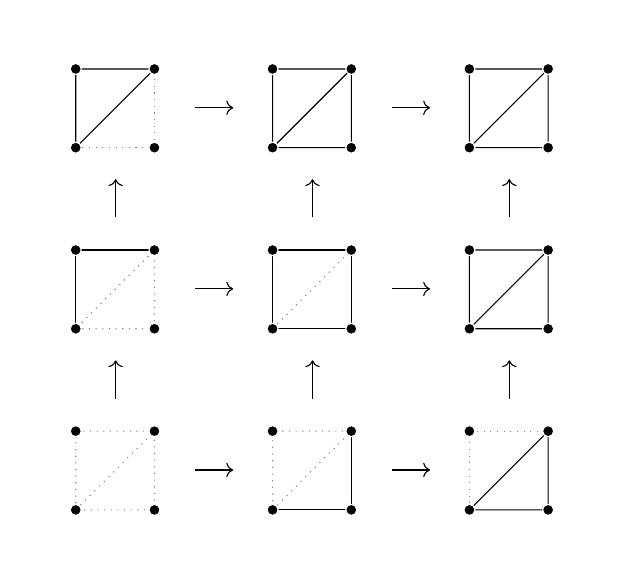
\begin{tikzpicture}[
        commutative diagrams/every diagram,
        anchor box/.style={minimum width=2.0cm, minimum height=1.8cm, anchor=south west, at={(-5mm, -4mm)}},
        bounding box/.style={},
        dot/.style={radius=2pt, draw=white, fill=black},
        spanning edge/.style={very thick, draw=green},
        cospanning edge/.style={very thick, draw=blue},
        hidden edge/.style={color=gray, dotted},
        edge/.style={draw=black},
        emph path/.style={
            start angle=90,
            end angle=400,
            radius=1.5mm,
            yshift=1.5mm,
            thick,
            arrows={->[length=0.7mm]},
            draw=orange
        },
        emph path label/.style={},
        baseline=(m-1-1.north)]
        \matrix[matrix anchor=west, column sep=5mm, row sep=5mm] at (0, 0) {
            \draw[hidden edge]
                (0, 0) -- (1, 0) -- (1, 1);
            \draw[edge] (0, 0) -- (0, 1) -- (1, 1) -- cycle;
            \path[dot]
                (0, 0) circle[]
                (1, 0) circle[]
                (0, 1) circle[]
                (1, 1) circle;
            \node[anchor box] (m-1-1) {};
            \&
            \draw[edge] (0, 0) -- (0, 1) -- (1, 1) -- (1, 0) -- cycle
                (0, 0) -- (1, 1);
            \path[dot]
                (0, 0) circle[]
                (1, 0) circle[]
                (0, 1) circle[]
                (1, 1) circle;
            \node[anchor box] (m-1-2) {};
            \&
            \draw[edge] (0, 0) -- (0, 1) -- (1, 1) -- (1, 0) -- cycle
                (0, 0) -- (1, 1);
            \path[dot]
                (0, 0) circle[]
                (1, 0) circle[]
                (0, 1) circle[]
                (1, 1) circle;
            \node[anchor box] (m-1-3) {};
            \\
            \draw[hidden edge]
                (0, 0) -- (1, 0) -- (1, 1) -- cycle;
            \draw[edge]
                (0, 0) -- (0, 1) -- (1, 1);
            \fill[dot]
                (0, 0) circle[]
                (1, 0) circle[]
                (0, 1) circle[]
                (1, 1) circle;
            \node[anchor box] (m-2-1) {};
            \&
            \draw[hidden edge]
                (0, 0) -- (1, 1);
            \draw[edge]
                (0, 0) -- (0, 1) -- (1, 1) -- (1, 0) -- cycle;
            \fill[dot]
                (0, 0) circle[]
                (1, 0) circle[]
                (0, 1) circle[]
                (1, 1) circle;
            \node[anchor box] (m-2-2) {};
            \&
            \draw[edge] (0, 0) -- (0, 1) -- (1, 1) -- (1, 0) -- cycle
                (0, 0) -- (1, 1);
            \fill[dot]
                (0, 0) circle[]
                (1, 0) circle[]
                (0, 1) circle[]
                (1, 1) circle;
            \node[anchor box] (m-2-3) {};
            \\
            \draw[hidden edge]
                (0, 0) -- (0, 1) -- (1, 1) -- (1, 0) -- cycle
                (0, 0) -- (1, 1);
            \path[dot]
                (0, 0) circle[]
                (1, 0) circle[]
                (0, 1) circle[]
                (1, 1) circle;
            \node[anchor box] (m-3-1) {};
            \&
            \draw[hidden edge]
                (0, 0) -- (1, 1) -- (0, 1) -- cycle;
            \draw[edge] (0, 0) -- (1, 0) -- (1, 1);
            \fill[dot]
                (0, 0) circle[]
                (1, 0) circle[]
                (0, 1) circle[]
                (1, 1) circle;
            \node[anchor box] (m-3-2) {};
            \&
            \draw[hidden edge]
                (0, 0) -- (0, 1) -- (1, 1);
            \draw[edge] (0, 0) -- (1, 0) -- (1, 1) -- cycle;
            \fill[dot]
                (0, 0) circle[]
                (1, 0) circle[]
                (0, 1) circle[]
                (1, 1) circle;
            \node[anchor box] (m-3-3) {};
            \\
        };
        \path[commutative diagrams/.cd, every arrow, every label]
            (m-3-1) edge (m-3-2)
            (m-3-1) edge (m-2-1)
            (m-3-2) edge (m-3-3)
            (m-3-2) edge (m-2-2)
            (m-3-3) edge (m-2-3)
            (m-2-1) edge (m-2-2)
            (m-2-1) edge (m-1-1)
            (m-2-2) edge (m-2-3)
            (m-2-2) edge (m-1-2)
            (m-2-3) edge (m-1-3)
            (m-1-1) edge (m-1-2)
            (m-1-2) edge (m-1-3);
    \end{tikzpicture}

    \caption{A $3\times 3$-filtration of simplicial complexes without a corresponding subfiltration of spanning trees in the sense of Proposition~\ref{proposition:PersistentFiltration}.}
    \label{figure:NoSubfiltration}
\end{figure}

\begin{example}
    \label{example:NoSubfiltrationOfST}
    If the poset $Q$ is not total, the existence of a subfiltration of spanning trees for any filtration over $Q$ is not guaranteed.
    A counterexample of such filtration over $\mathbb N^2$ is depicted in Figure~\ref{figure:NoSubfiltration}.
    This failure of existence is also reflected in the fact that the decomposition structure of persistence modules over non-totally ordered sets is not trivial \cite{CarlssonZomorodian2009}.
\end{example}

\begin{definition}[Cofiltrations of spanning trees]
    \label{definition:CofST}
    Let $(T^q)_{q \in Q}$ be a family of simplicial complexes such that $T^q$ is a spanning tree of $X^q$ for any $q \in Q$.
    The family $(T^q)_{q \in Q}$ is a \emph{cofiltration of spanning trees} of $X$ if $X^q \setminus T^q \subseteq X^{q'} \setminus T^{q'}$ set-theoretically for any pair $q \leq q'$ in $Q$.
\end{definition}

A similar but more general notion of cofiltrations was introduced in \cite{PatelRask2022}.

\begin{lemma}%
    \label{lemma:ClassicComplementInclusion}
    Let $(X, \mathord\preceq)$ be an ordered simplicial complex and $A$ a subcomplex of $X$.
    Interpret $A$ as an ordered simplicial complex, with ordering given by the restriction of $\mathord\preceq$.
    For order-minimal spanning trees $T_A$ and $T_X$ of $A$ and $Y$, respectively, it holds $A \setminus T_A \subseteq X \setminus T_X$ set-theoretically.

    \begin{proof}
        Let $e \in A \setminus T_A$.
        Then, we find $c = \sum_{i = 1}^k \lambda_i e_i \in C_1(T_A)$ such that the chain $z = c - e$ is a cycle in $A$.
        By Lemma~\ref{proposition:LeadingSimplexComplement}, the leading simplex of $z$ must be contained in $A \setminus T_A$, and the only possibility is $\LS(z) = e$.
        Since $T_X$ is an order-minimal spanning tree of $X$, it further follows that $\LS(z) \in X \setminus T_X$.
        Hence, we have $e \in X \setminus T_X$.
    \end{proof}    
\end{lemma}

Our main result in this section is that we can use the above lemma to obtain, for every filtration of finite simplicial complexes over a finite poset, a corresponding cofiltration of spanning trees, cf.\ Theorem~\ref{theorem:IntroMainResult}.

\begin{theorem}
    \label{theorem:MainResult}
    Let $X = (X^q)_{q \in Q}$ be a filtration of finite simplicial complexes.
    Then, there exists a cofiltration of spanning trees $T$ of $X$, i.e.\ a family $T = (T^q)_{q \in Q}$ of simplicial complexes with $X^q \setminus T^q \subseteq X^{q'} \setminus T^{q'}$ for any pair $q \leq q' \in Q$.

    \begin{proof}
        We choose for any $q \in Q$ an order-minimal spanning tree $T^q$ of $X^q$, which exists since $X^q$ is finite.
        Let $q \leq q' \in Q$.
        We know by assumption that $X^q$ is a subcomplex of $X^{q'}$.
        Thus, by Lemma~\ref{lemma:ClassicComplementInclusion}, we have $X^q \setminus T^q \subseteq X^{q'} \setminus T^{q'}$.
        Hence, $(T^q)_{q \in Q}$ is a cofiltration of spanning trees of $(X^q)_{q \in Q}$.
    \end{proof}    
\end{theorem}

Lastly, we show that we can extend the above result in a functorial fashion for order- and dimension-preserving simplicial maps.
A morphism of simplicial complexes~$f \colon X \to Y$ is called \emph{dimension-preserving} if $\dim \sigma = \dim f(\sigma)$.
Let $\Simp_{\ord, \dim}$ denote the subcategory of ordered simplicial complexes with dimension- and order-preserving simplicial maps as morphisms.

\begin{definition}
    Let $A \subseteq X$ be a pair of simplicial complexes and $n \in \mathbb N$.
    The \emph{$n$-difference of $X$ and $A$} is the set
    \[ X \boxminus_n A = X_0 \cup \dotsc \cup X_{n-1} \cup (X_n \setminus A_n) \text. \]
\end{definition}

It is immediately clear that $X \boxminus_n A$ is again a simplicial complex contained in $X$.
Further, we note that the $(n-1)$-skeleton of $X \boxminus_n A$ coincides with the $(n-1)$-skeleton of $X$.

\begin{theorem}%
    \label{theorem:ComplementInclusionFunctorial}
    Let $f\colon (X, \mathord\leq_X) \to (Y, \mathord\leq_Y)$ be an order- and dimension-preserving simplicial map.
    Suppose that $T_X$ is an order-minimal spanning tree of $X$ and $T_Y$ is an order-minimal spanning tree of $Y$.
    Then, $f(X \boxminus_1 T_X) \subseteq Y \boxminus_1 T_Y$.
    
    Hence, $f$ restricts to a simplicial map $X \boxminus_1 T_X \to Y \boxminus_1 T_Y$.

    \begin{proof}
        Let $\lambda_1, \dotsc, \lambda_k \neq 0$ and $\sigma_1, \dotsc, \sigma_k$ be distinct $1$-simplices in $X$ satisfying $\sigma_1 \preceq_X \dotsb \preceq_X \sigma_k$.
        That is, for the chain $c = \lambda_1 \sigma_1 + \dotsb + \lambda_k \sigma_k$ we have $\LS(c) = \sigma_k$.
    
        Since $f$ is order-preserving, it follows $f(\sigma_1) \preceq_Y \dotsb \preceq_Y f(\sigma_k)$.
        Moreover, since $f$ is dimension-preserving, every simplex $f(\sigma_i)$ is an $1$-simplex for $i \in \{ 1, \dotsc, k \}$.
        
        Let $f_\sharp\colon C_1(X) \to C_1(Y)$ be the associated homomorphism of chain modules of~$f$.
        Therefore, we have $f_\sharp(c) = \lambda_1 f(\sigma_1) + \dotsb + \lambda_k f(\sigma_k)$.
        Hence, $\LS(f_\sharp(c)) = f(\sigma_k) = f(\LS(c))$.
    
        Now, let $\sigma$ be an $1$-simplex in $X$ but not in $T_X$.
        Then, we choose a chain $c$ in $T_X$ such that $c - \sigma \in Z_1(X)$.
        Since the spanning tree $T_X$ is order-minimal, we have $\LS(c - \sigma) \in X \setminus T_X$.
        Thus, it holds $\LS(c - \sigma) = \sigma$.
    
        By the considerations above, we have $\LS(f_\sharp(c - \sigma)) = f(\LS(c - \sigma)) = f(\sigma)$.
        Since $T_Y$ is also order-minimal and $f_\sharp(c - \sigma)$ is by definition a non-zero $1$-cycle in $Y$, it follows $\LS(f_\sharp(c - \sigma)) \in Y \setminus T_Y$.
        Hence, $f(\sigma) \in Y \boxminus_1 T_Y$, which proves the assertion.
    \end{proof}    
\end{theorem}

\begin{remark}%
    \label{remark:MonoIsDimPreserv}
    Every monomorphism of simplicial complexes is necessarily dimension-preserving.
    Hence, if $f\colon (X, \mathord\leq_X) \to (Y, \mathord\leq_Y)$ is a monomorphism, it follows $f(X \setminus T_X) \subseteq Y \setminus T_Y$.
\end{remark}

\begin{example}
    Let $X$ be a wedge of two triangles and $Y$ a single triangle.
    A simplicial map from $X$ into $Y$ that sends each triangle in $X$ onto the triangle $Y$ is dimension-preserving but not injective.
\end{example}

\begin{corollary}%
    \label{corollary:EndoFunc}
    There is an endofunctor $\tau_1\colon \Simp_{\ord, \dim} \to \Simp_{\ord, \dim}$ defined as follows:
    For $(X, \mathord\preceq_X)$ an ordered simplicial complex, let $T_X$ be the unique order-minimal spanning tree of $X$.
    Then, define $\tau_1(X, \mathord\preceq_X) = (X \boxminus_1 T_X, \mathord\preceq_X)$.

    For a morphism $f\colon (X, \mathord\preceq_X) \to (Y, \mathord\preceq_Y)$ in $\Simp_{\ord, \dim}$, let $T_Y$ be the order-minimal spanning tree of $Y$.
    Define the morphism $\tau_1(f)\colon X \boxminus_1 T_X \to Y \boxminus_1 T_Y$ to be the underlying simplicial map of $f$ formally restricted to $X \boxminus_1 T_X$, interpreted as a morphism in $\Simp_{\ord, \dim}$.

    In particular, this functor is faithful but not full in general.
\end{corollary}

\begin{remark}
    Let $A \subseteq X$ be a simplicial pair and let $i\colon A \to X$ denote the canonical inclusion map.
    Further, we assume that $X$ is endowed with a simplicial order~$\preceq_X$ and we endow $A$ with the restriction of $\preceq_X$ as simplicial order.
    Under this assumption, we see that $i$ is an order-preserving simplicial map $(A, \preceq_X) \to (X, \preceq_X)$.
    
    Moreover, it follows from Remark~\ref{remark:MonoIsDimPreserv} that $i$ is also dimension-preserving.
    Thus, Corollary~\ref{corollary:EndoFunc} implies that there is an order- and dimension-preserving simplicial map $\tau_1(i)\colon (A \boxminus_1 T_A, \mathord\preceq_X) \to (X \boxminus_1 T_X, \mathord\preceq_X)$, where $T_A$ is the order-minimal spanning tree of~$A$ and $T_X$ is the order-minimal spanning tree of~$X$.

    From this result, it directly follows that $A_1 \setminus T_A$ is a subset of $X_1 \setminus T_X$.
    Hence, Corollary~\ref{corollary:EndoFunc} is a vast generalization of Lemma~\ref{lemma:ClassicComplementInclusion} and Theorem~\ref{theorem:MainResult}.
\end{remark}

\section{\texorpdfstring{$R$}{R}-spans of persistence modules}%
\label{section:RSpans}
Let $R$ be a principal ideal domain and $Q = (Q, \mathord\leq)$ a poset.
Denote by $U_0$ the forgetful functor $\Mod{R} \to \Set$ sending an $R$-module to its underlying set.
We consider the forgetful functor
\begin{align*}
    U_{Q}\colon \Mod{R}^Q &\longrightarrow \Set^Q \text, \\
    M &\longmapsto U_0 \circ M \text.
\end{align*}

The functor~$U$ sending an $R$-module to its underlying set is right-adjoint to the $R$-span functor $R\colon \Set \to \Mod{R}$, which for any set $B$ assigns the free $R$-module $R(B)$ with basis $B$ to the set $B$.
We now show that the adjunction $U \dashv R$ extends to an adjunction of $U_{Q}$.

Let $\eta_{X, M}\colon \Hom_{\Mod{R}}(R(X), M) \to \Hom_{\Set}(X, U(M))$ be the natural transformation in $X \in \Set^Q$ and $M \in \Mod{R}^Q$ associated to the adjunction.
We consider the functor $R_{Q}\colon \Set^{Q} \to \Mod{R}^{Q}$ defined on a persistent set~$X$ by $R_{Q}(X) = R \circ X$, and we claim that $R_{Q}$ is the left adjoint of $U_{Q}$.

For any persistent set $X$ and persistence module $M$ we define the map
\begin{align*}
    \theta_{X, M}\colon \Hom_{\Mod{R}^{Q}}(R_{Q}(X), M) &\longrightarrow \Hom_{\Set^{Q}}(X, U_{Q}(M)) \text, \\
    (\alpha_q)_{q \in Q} &\longmapsto (\eta_{X(q), M(q)}(\alpha_q))_{q \in Q} \text.
\end{align*}
It is easy to see that this is natural in $X \in \Set^{Q}$ and $M \in \Mod{R}^{Q}$.
Moreover, $\theta_{X,M}$ is an isomorphism with inverse given by the map
\begin{align*}
    \theta_{X,M}^{-1}\colon \Hom_{\Set^Q}(X, U_Q(M)) &\longrightarrow \Hom_{\Mod{R}^Q}(R_Q(X), M) \text, \\
    (\beta_q)_{q \in Q} &\longmapsto (\eta_{X(q), M(q)}^{-1}(\beta_q))_{q \in Q} \text.
\end{align*}

The functor $R_{Q}\colon \Set^{Q} \to \Mod{R}^{Q}$ defined in this context is called the \emph{persistent $R$-span functor}.
These considerations prove the following lemma.

\begin{lemma}
    The forgetful functor $U_{Q}\colon \Mod{R}^{Q} \to \Set^{Q}$ admits a left-adjoint functor, namely $R_{Q}$.
    In particular, $U_{Q}$ preserves limits, products, and finite coproducts and, dually, $R_{Q}$ preserves colimits, coproducts, and finite products \cite{MacLane1978}.
\end{lemma}

\begin{definition}
    Let $\mathcal B$ be a set consisting of persistent sets.
    A persistence module~$M\colon Q \to \Mod{R}$ is \emph{$\mathcal B$-decomposable} if there exists a family $(B_i)_{i \in I}$ of elements of $\mathcal B$ such that
    \[ M \cong \bigoplus_{i \in I} \mathop{R_{Q}}(B_i) \text. \]
\end{definition}

Specifically, we consider the family $\mathcal U$ of principal persistent sets, defined as follows.
A subset $U$ of the poset~$Q$ is an \emph{upper set} (also called an \emph{order coideal} in order theory) if for all $q \in U$ and $q' \in Q$ with $q \leq q'$ it follows $q' \in U$.
Given such upper set $U \subseteq Q$, the associated \emph{principal persistent set} is the persistent set $\pt[U]\colon Q \to \Set$ with $\pt[U](q) = \{ \ast \}$ if $q \in U$ and $\pt[U](q) = \emptyset$ otherwise, and $\pt[U](q \leq q')$ the identity map unless $q \notin U$.

With these notions, we define
\[ \mathcal U = \mathcal U_{Q} = \{ \pt[U] \mid \text{$U$ an upper subset of $Q$} \} \text. \]
If a persistence module $M\colon Q \to \Mod{R}$ is $\mathcal U$-decomposable, we say that $M$ is \emph{upper set decomposable} (USD).
That is, $M$ is upper set decomposable if and only if there exists a family $(U_i)_{i \in I}$ of upper subsets of $Q$ such that $M = \bigoplus_{i \in I} R[U_i]$.
Moreover, if $U$ is an upper set, the module $R[U] = R_{Q}(\pt[U])$ is the \emph{upper set module} of $U$.

\begin{proposition}%
    \label{proposition:SemiFree}
    Let $B\colon Q \to \Set$ a functor.
    For $q \in Q$, denote by $\iota_q\colon B(q) \to \colim B$ the colimit injection.
    Then the following assertions are equivalent:
    \begin{enumerate}[label=(\roman*)]
        \item\label{proposition:SemiFree:a1} For every $q \in Q$, the map $\iota_q$ is injective.
        \item\label{proposition:SemiFree:a2} The persistence module $\mathop{R_Q} B$ is upper set decomposable.
        \item\label{proposition:SemiFree:a3} For every $q \in Q$, the colimit injection $\iota'_q\colon \mathop{R_Q} B(q) \to \colim \mathop{R_Q} B$ is a monomorphism.
    \end{enumerate}

    \begin{proof}
        \textbf{\ref{proposition:SemiFree:a1} $\implies$ \ref{proposition:SemiFree:a2}:}
        We define the persistent set $B'\colon Q \to \Set$ as follows:
        For $q \in Q$, let $B'(q) = \iota_q(B(q))$.
        
        Then, for an ordered pair $q \leq q'$ in $Q$ and every $x \in B'(q)$ we have $x \in B'(q')$ since $\iota_q = \iota_{q'} \circ B(q \leq q')$ holds.
        Therefore, the map $B'(q \leq q')\colon \iota_q(B(q)) \to \iota_{q'}(B(q'))$ can be chosen as the inclusion.
        
        Moreover, $B'$ is isomorphic to $B$ by construction.
        For every $q \in Q$, the map
        \[ B(q) \to B'(q) \text, \qquad b \mapsto \iota_q(b) \text, \]
        is bijective by the injectivity of $\iota_q$.
        Thus, $B' \cong B$.
    
        Further, $B'$ is upper set decomposable since we can decompose $B'$ into the coproduct of $\pt[U_x]$ over any $x \in \colim B$, where $U_x = \{ q \in Q \mid x \in B'(q) \}$ is an upper set of $Q$ by construction.
    
        \textbf{\ref{proposition:SemiFree:a2} $\implies$ \ref{proposition:SemiFree:a3}:}
        Let $(U_i)_{i \in I}$ be a family of upper sets of $Q$ such that $\mathop{R_Q} B = \bigoplus_{i \in I} R[U_i]$.
        Since every upper set module $R[U_i]$ admits monic colimit injections $R[U_i](q) \to \colim R[U_i]$ for any $q \in Q$, it follows that $\mathop{R_Q} B$ also admits monic colimit injections as claimed.
    
        \textbf{\ref{proposition:SemiFree:a3} $\implies$ \ref{proposition:SemiFree:a2}:}
        Suppose that there exists some $q \in Q$ such that $\iota_q$ is not injective.
        Then, there are $b, b' \in B(q)$ such that $b \neq b'$ and $\iota_q(b) = \iota_q(b')$.
        Thus, $b - b' \in R_Q B(q)$ is a non-zero element of the kernel of $\iota'_q$ since $R_Q$ preserves colimits.
        Hence, $\iota'_q$ is not injective and thus not a monomorphism.
    \end{proof}    
\end{proposition}

\begin{remark}
    Results similar to Proposition~\ref{proposition:SemiFree} were established in \cite{ChachólskiScolamieroVaccarino2017}.
    A functor $B\colon Q \to \Mod{R}$ is a \emph{multifiltration} if the structure maps of $B$ are monomorphisms.
    For the poset $Q = \mathbb N^d$ (or more generally for $Q$ a lattice), the conditions of Proposition~\ref{proposition:SemiFree} are equivalent to the condition that the functor $B$ is a multifiltration, cf. \cite[Proposition~3.3]{ChachólskiScolamieroVaccarino2017}.
    Moreover, any non-trivial multifiltration $B$ is uniquely decomposable into indecomposables and the indecomposable multifiltrations over $\mathbb N^d$ are precisely the upper set modules \cite[Proposition~3.1, Corollary~3.2]{ChachólskiScolamieroVaccarino2017}.
    In this sense, Proposition~\ref{proposition:SemiFree} is a generalization of \cite[Proposition~3.1]{ChachólskiScolamieroVaccarino2017}.
\end{remark}
\begin{example}
    Let $U = \{ (a, b) \in \mathbb Z^2 \mid a + b \geq 0 \}$.
    This is clearly an upper set of $\mathbb Z^2$.
    However, the upper set module $R[U]$ is not finitely generated, since we need a generator in each $(a, -a)$ for $a \in \mathbb Z$ to cover $U$ by principal upper sets of $\mathbb Z^2$.
\end{example}

\section{Generating  persistent first homology}
\label{section:GeneratingH1}
Let $X = (X^q)_{q \in Q}$ be a $Q$-filtration of simplicial complexes and $(T^q)_{q \in Q}$ a filtration of spanning trees of $X$.
Then, we have seen in Proposition~\ref{proposition:PersistentFiltration} that we can describe $Z_1(X)$ as the quotient persistence module $C_1(X, T) = C_1(X) / C_1(T)$.

Since $C_1(X, T)$ has monomorphic colimit injections, it follows that $Z_1(X)$ is, in this case, upper set decomposable.
This results in a decomposition $Z_1(X) \cong \bigoplus_{i \in I} R[U_i]$ for a family $(U_i)_{i \in I}$ of upper sets of $Q$.

All of this depends on the requirement that there exists a filtration of spanning trees for $(X^q)_{q \in Q}$.
We have seen in Example~\ref{example:NoSubfiltrationOfST} that this is not always the case.
The existence of such filtration of spanning trees fails even for a $3 \times 3$ sublattice of $\mathbb N^2$.

As an alternative for the general case, we propose in this section a technique to determine upper sets $(U_i)_{i \in I}$ together with an epimorphism $\bigoplus_{i \in I} R[U_i] \to Z_1(X)$ by exploiting the properties of order-minimal spanning trees, namely Theorem~\ref{theorem:MainResult}.

We assume that the poset $Q$ and the simplicial complex $\bigcup_{q \in Q} X^q$ are finite and endowed with a simplicial order~$\preceq$.
Then, for every $q \in Q$ we interpret the subcomplex $X^q$ as the ordered simplicial complex $(X^q, \mathord\preceq)$, which naturally admits an injective order-preserving simplicial map into $(X, \mathord\preceq)$.
Using the simplicial order on $X^q$, we choose the uniquely determined order-minimal spanning tree $T^q$ of $(X^q, \mathord\preceq)$.
Since $X^q$ is a finite simplicial complex, the existence of $T^q$ is guaranteed.

Then, it follows from Theorem~\ref{theorem:MainResult} that $X^q \boxminus_1 T^q$ is a subcomplex of $X^{q'} \boxminus_1 T^{q'}$.
Moreover, when $T^\infty$ is the order-minimal spanning tree of $X^\infty = \bigcup_{q \in Q} X^q$ endowed with $\preceq$, we also have $X^q \boxminus_1 T^q \subseteq X^\infty \boxminus_1 T^\infty$ for any $q \in Q$.

Let $\sigma \in X^\infty \boxminus_1 T^\infty$ be a 1-simplex.
We shall write $\Supp_{X \boxminus_1 T}(\sigma) = \{ q \in Q \mid \sigma \in X^q \boxminus_1 T^q \}$.
For every $q \in Q$ such that $\sigma \in \Supp_{X \boxminus_1 T}(\sigma)$ we consider the $R$-module isomorphism $j^q\colon Z_1(X^q) \to C_1(X^q, T^q)$.
We define the persistent set $B_\sigma = (B_\sigma^q)_{q \in Q}$ by $B_\sigma^q = \{ j^{-1}_{q'}(\sigma) \mid q' \in (- \infty, \sigma] \cap \Supp_{X \boxminus_1 T}(\sigma) \}$ and structure maps given by inclusions.

Finally, let $M$ be the $R$-span of the persistent set $\coprod_{\sigma} B_\sigma$, i.e.\ $M = R_Q(\coprod_\sigma B_\sigma) \cong \bigoplus_\sigma R_Q B_\sigma$ where $\sigma$ ranges over each $1$-simplex in $X^\infty \boxminus_1 T^\infty$.

\begin{theorem}%
    \label{theorem:GenH1}
    The module $M$ as constructed above is upper set decomposable and admits an epimorphism onto $Z_1(X)$.

    \begin{proof}
        The persistent set $B = (B^q)_{q \in Q} =  \coprod_{\sigma} B_\sigma$ is given by
        \[ B^q = \{ (\sigma, j^{-1}_{q'}(\sigma)) \mid \sigma \in X^q \boxminus_1 T^q,\ q' \in (-\infty, \sigma] \cap \Supp_{X \boxminus_1 T}(\sigma) \} \text. \]
        We define the persistent map $\varphi = (\varphi^q)_{q \in Q} \colon B \to \mathop{U_Q} Z_1(X)$ as follows:
        For $(\sigma, z) \in B^q$, $z$~is a cycle of $X^{q'}$ for some $q' \in Q$ satisfying $q' \leq q$.
        Thus, $z$~is a cycle in $X^q$, and we define $\varphi^q(\sigma, z) = z \in Z_1(X^q)$.
    
        We have a basis $\mathcal B_q = \{ j_q^{-1}(\sigma + C_1(T^q)) \mid \sigma \in X^q \boxminus_1 T^q \mid |\sigma| = 2 \}$ of $Z_1(X^q)$.
        By construction, the image of $\varphi^q$ contains $\mathcal B_q$.
        Thus, the uniquely determined homomorphism $\tilde \varphi^q\colon R B \to Z_1(X^q)$ is an epimorphism.
    
        It follows that the uniquely determined persistent homomorphism $\varphi\colon R_Q \to Z_1(X)$ is an epimorphism in each component.
        Hence, $\varphi$ is an epimorphism in the category of persistence modules.
    \end{proof}    
\end{theorem}

\section{Higher-dimensional spanning complexes}%
\label{section:HigherDimensionalSpanningSubcomplexes}

In the previous sections, we discussed spanning trees of simplicial complexes, which allow us to determine the $1$-dimensional cycle modules of simplicial complexes by inspecting $1$-dimensional relative chain modules.
An open question is whether there is a similar, easily computable type of subcomplex such that for a dimension~$n \in \mathbb N$ we can determine $n$-dimensional cycle modules in a similar manner by inspecting $n$-dimensional relative chain modules.

As a first step towards an answer of this question, we consider in this section a generalization of spanning trees to higher dimensions by merely generalizing Definition~\ref{definition:SpanningTree}.
\begin{definition}%
    \label{definition:SpanningSubcomplex}
    Let $X$ be a simplicial complex and $n > 0$.
    A subcomplex~$A$ of~$X$ is an \emph{$n$-spanning complex} of~$X$ if the following conditions hold:
    \begin{enumerate}[label=(\roman*)]
        \item\label{definition:SpanningSubcomplex:c1} $\skel_{n-1}(A) = \skel_{n-1}(X)$.
        \item\label{definition:SpanningSubcomplex:c2} The boundary homomorphism $\partial_n\colon C_n(A) \to C_{n-1}(A)$ is injective.
        \item\label{definition:SpanningSubcomplex:c3} $B_{n-1}(A) = B_{n-1}(X)$.
    \end{enumerate}
\end{definition}

This definition directly generalizes the notion of a spanning tree defined in Definition~\ref{definition:SpanningTree} by replacing the dimensions by an fixed but arbitrary $n \in \mathbb N$.

\begin{remark}
    For $n = 1$, every spanning tree is an $n$-spanning complex.
\end{remark}

\begin{proposition}%
    \label{proposition:NSSMain}
    Let $A$ be an $n$-spanning complex of $X$.
    Then the homomorphism
    \begin{align*}
        j\colon Z_n(A) &\longrightarrow C_n(X, A) \text, \\
        z &\longmapsto z + C_n(A) \text,
    \end{align*}
    is an isomorphism of $R$-modules.

    \begin{proof}
        The proof is analogous to Theorem~\ref{theorem:SpanningTreeMain}.
        The injectivity of $j$ follows from $Z_n(A) = 0$ and the surjectivity of $j$ follows from $B_{n-1}(X) = B_{n-1}(A)$ together with $Z_n(A) = 0$.
    \end{proof}    
\end{proposition}

\begin{theorem}[Existence of $n$-spanning complexes]%
    \label{theorem:ExistenceNSS}
    For any simplicial complex~$X$ and any $n \in \mathbb N$ there exists a subcomplex $A$ such that $Z_n(A) = 0$ and $B_{n-1}(A) = B_{n-1}(X)$, i.e.\ $X$ admits an $n$-spanning complex.

    \begin{proof}
        Let $\mathcal A_X = \{ A \subseteq X \mid \text{$A$ is a subcomplex s.t.\ $Z_n(A) = 0$} \}$.
        For every subset $\mathcal A' \subseteq \mathcal A_X$ that is totally ordered by set inclusion, we consider the subcomplex $\bigcup \mathcal A = \bigcup_{A \in \mathcal A'} A$ of $X$.
        We have $Z_n(\bigcup \mathcal A') = 0$:
        Let $z$ be an $n$-chain in $\bigcup \mathcal A'$ such that $\partial_n z = 0$.
        Then, there are non-zero $\lambda_1, \dotsc, \lambda_k \in R$ and distinct $n$-simplices $\sigma_1, \dotsc, \sigma_k$ in $\bigcup \mathcal A'$ such that $z = \lambda_1 \sigma_1 + \dotsb + \lambda_k \sigma_k$.
        Then, we can choose $A_1, \dotsc, A_k \in \mathcal A'$ such that $\sigma_i \in A_i$ for $i \in \{ 1, \dotsc, k \}$.
        Since $\mathcal A'$ is totally ordered by set inclusion there exists an $i_0 \in \{ 1, \dotsc, k \}$ such that $A_i \subseteq A_{i_0}$ for all $i \in \{ 1, \dotsc, k \}$.
        Thus, $z$ is actually an $n$-chain in $B_{i_0} \in \mathcal A'$.
        Since $B_{i_0}$ satisfies $Z_1(B_{i_0}) = 0$ by assumption, $z = 0$.
    
        Therefore, every totally ordered subset of $\mathcal A_X$ admits an upper bound in $\mathcal A_X$.
        It follows from Zorn's lemma that there exists $A \in \mathcal A_X$ that is maximal w.r.t.\ set inclusion.
    
        It remains to prove that such maximal $A$ in $\mathcal A_X$ satisfies $B_{n-1}(A) = B_{n-1}(X)$, i.e.\ $B_{n-1}(X) \subseteq B_{n-1}(A)$.
        In particular, it suffices to prove that for every $n$-simplex $\sigma$ in $X$ there exists an $n$-chain $c$ in $A$ such that $\partial_n c = \partial_n \sigma$.
        Let $\sigma$ be an $n$-simplex in $X$.
        If $\sigma \in A$, then trivially $\partial_n \sigma \in B_{n-1}(A)$.
        Thus, we consider only the case that $\sigma$ is not in $A$.
        Then, we can consider the subcomplex $A' = A \cup \{ \sigma \}$ of $X$.
        Since $A$ is maximal by construction in $\mathcal A_X$ and $A \subsetneq A'$, it follows that $A'$ cannot be contained in $\mathcal A_X$.
        That is, $Z_n(A')$ cannot be trivial.
        
        Therefore, there exists an $n$-cycle $z = \mu \sigma + c$ in $A'$ with $\mu \in \{ 1, -1 \}$ and $c$ an $n$-chain in $A$.
        We can assume without loss of generality that $\mu = 1$.
        But then we have $\partial_n \sigma = \partial_n c \in B_{n-1}(A)$.
        Hence, $B_{n-1}(X) \subseteq B_{n-1}(A)$.
    \end{proof}    
\end{theorem}

\emergencystretch=1em
\printbibliography
\end{document}
